%% ══════════════════════════════════════════════════════════════
%%  CHAPTER 5 — AUTONOMOUS JOURNAL SYSTEM
%% ══════════════════════════════════════════════════════════════
\chapter{Autonomous Journal System}
\label{ch:journal}

\section{What Makes It a Journal}
\label{sec:journal:definition}

\autoscholar implements what can be described as the first \textbf{autonomous academic journal}---a system that continuously generates, reviews, and publishes research papers without human editorial oversight.
The term ``journal'' is used deliberately to evoke the key characteristics shared with traditional academic publishing:

\begin{description}
  \item[Continuous publication.] Papers are generated and published on a regular cadence, similar to a journal's issue schedule, but at a much higher frequency (one paper per hour vs. quarterly or monthly issues).

  \item[Peer review.] Every paper undergoes AI-powered peer review (\popper) before publication, with explicit acceptance/rejection criteria.

  \item[Persistent identifiers.] Published papers receive AutoScholar Identifiers (ASIDs) analogous to DOIs, enabling stable references.

  \item[Quality thresholds.] Papers scoring below 45/100 on the peer review are rejected, enforcing a minimum quality standard.

  \item[Archival storage.] All papers, including rejected ones, are stored with full source code, data, and reproducibility packages.

  \item[Public access.] Published papers are accessible via the web interface and REST API.
\end{description}

However, it is critical to note that this is a \emph{machine-generated} journal with no human reviewers, editors, or authors.
The quality standards, while enforced systematically, are evaluated by the same class of AI model that generated the content.

\section{Scheduling Architecture}
\label{sec:journal:scheduling}

\subsection{The AutoPaper Scheduler}

The scheduler (\file{autoPaperScheduler.ts}, 1,285 lines) is the heartbeat of the autonomous journal.
It manages the full lifecycle of paper generation runs.

\subsubsection{Configuration}

The scheduler exposes a comprehensive configuration interface:

\begin{table}[H]
\centering
\caption{Scheduler configuration parameters.}
\label{tab:scheduler-config}
\begin{tabularx}{\textwidth}{lXl}
\toprule
\textbf{Parameter} & \textbf{Description} & \textbf{Default} \\
\midrule
\texttt{enabled} & Whether the scheduler is active & \texttt{true} \\
\texttt{cadenceMinutes} & Time between paper generation starts & 60 \\
\texttt{maxParallel} & Maximum concurrent paper generations & 3 \\
\texttt{selectionMode} & Prompt selection strategy & \texttt{sequential} \\
\texttt{popperThreshold} & Minimum peer review score for publication & 45 \\
\texttt{heartbeatTimeout} & Seconds before a run is considered stalled & 300 \\
\texttt{cleanupEnabled} & Auto-cleanup of stale runs & \texttt{true} \\
\texttt{maxConsecutiveFailures} & Failures before auto-pausing & 5 \\
\bottomrule
\end{tabularx}
\end{table}

\subsubsection{Lifecycle States}

Each pipeline run transitions through a defined state machine:

\begin{figure}[H]
\centering
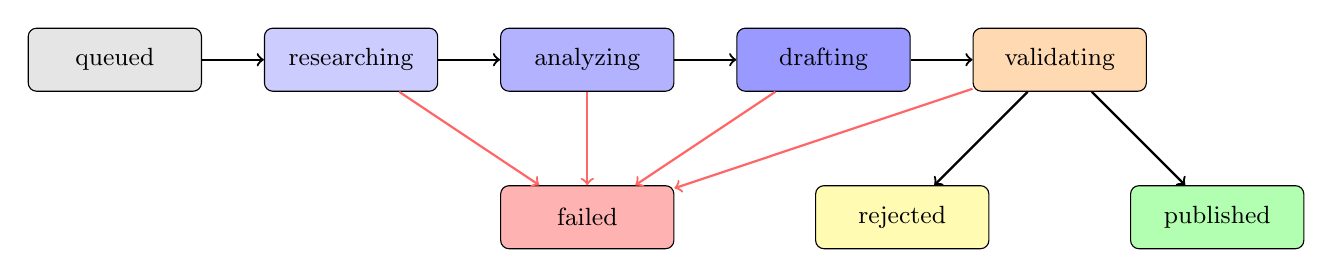
\begin{tikzpicture}[
  state/.style={draw, rounded corners=3pt, minimum width=2.2cm, minimum height=0.8cm, align=center, font=\small},
  arrow/.style={->, thick},
  fail/.style={->, thick, red!60},
]

\node[state, fill=gray!20] (queued) at (0,4) {queued};
\node[state, fill=blue!20] (research) at (3,4) {researching};
\node[state, fill=blue!30] (analyze) at (6,4) {analyzing};
\node[state, fill=blue!40] (draft) at (9,4) {drafting};
\node[state, fill=orange!30] (validate) at (12,4) {validating};
\node[state, fill=green!30] (published) at (14,2) {published};
\node[state, fill=yellow!30] (rejected) at (10,2) {rejected};
\node[state, fill=red!30] (failed) at (6,2) {failed};

\draw[arrow] (queued) -- (research);
\draw[arrow] (research) -- (analyze);
\draw[arrow] (analyze) -- (draft);
\draw[arrow] (draft) -- (validate);
\draw[arrow] (validate) -- (published);
\draw[arrow] (validate) -- (rejected);
\draw[fail] (research) -- (failed);
\draw[fail] (analyze) -- (failed);
\draw[fail] (draft) -- (failed);
\draw[fail] (validate) -- (failed);

\end{tikzpicture}
\caption{Pipeline run state machine.}
\label{fig:run-states}
\end{figure}

\subsubsection{Parallel Execution}

The scheduler supports up to 3 concurrent paper generations.
Before starting a new run, it checks:

\begin{enumerate}
  \item The number of active runs (status $\in$ \{queued, researching, analyzing, drafting, validating\}).
  \item If active runs $\geq$ \texttt{maxParallel}, the new run is deferred to the next cadence tick.
  \item Each run executes independently with its own session, governor state, and checkpoint.
\end{enumerate}

\subsection{Heartbeat Monitoring}

Every active run updates its heartbeat timestamp every 10 seconds.
The scheduler monitors heartbeats and:

\begin{itemize}
  \item Marks runs as \texttt{failed} if no heartbeat is received for \texttt{heartbeatTimeout} seconds (default: 300s = 5 minutes).
  \item Logs stale run detection for debugging.
  \item On server restart, force-fails all active runs to prevent zombie processes.
\end{itemize}

\subsection{Admin Controls}

Administrators have full control over the scheduler via the admin API:

\begin{itemize}
  \item \textbf{Enable/disable} the scheduler globally.
  \item \textbf{Update configuration} (cadence, parallel limit, selection mode, thresholds).
  \item \textbf{Trigger} immediate paper generation (random or custom prompt).
  \item \textbf{Abort} running papers by run ID.
  \item \textbf{Resume} failed runs from checkpoints.
  \item \textbf{Cleanup} stale or orphaned runs.
  \item \textbf{View} active run status and real-time progress.
\end{itemize}

\section{Quality Control}
\label{sec:journal:quality}

\subsection{Multi-Layer Quality Assurance}

Quality is enforced at multiple pipeline stages:

\begin{enumerate}
  \item \textbf{Prompt quality:} The 1,000+ entry prompt bank is curated with specific, publishable research questions. Prompts are enhanced by the research prompt upgrader.

  \item \textbf{Data quality:} The \governor monitors data collection and flags empty datasets, missing columns, and high NaN ratios. The \texttt{conservative} profile adds extra validation steps.

  \item \textbf{Analysis quality:} The system prompt mandates robustness checks, alternative specifications, and subsample analysis. The \governor enforces figure count limits.

  \item \textbf{Writing quality:} The JF Writing Style Directive enforces publication-quality prose with banned words, section conventions, and an 8-pass verification checklist.

  \item \textbf{Compilation quality:} The \LaTeX{} sanitizer and iterative repair loop ensure compilable output.

  \item \textbf{Peer review:} \popper evaluates 6 dimensions and issues a publication verdict.
\end{enumerate}

\subsection{Quality Metrics}

The system tracks the following quality metrics per paper:

\begin{itemize}
  \item Popper overall score (0--100).
  \item Popper dimension scores (originality, methodology, results, writing, references, reproducibility).
  \item Word count and section count.
  \item Figure count and \LaTeX{} line count.
  \item Governor confidence at publication time.
  \item Number of governor interventions.
  \item Number of Python error recoveries.
  \item Number of \LaTeX{} compilation attempts.
\end{itemize}

\subsection{Publication Threshold}

The configurable publication threshold (default 45/100) represents the minimum Popper score required for publication.
This threshold was calibrated based on early runs:

\begin{itemize}
  \item Papers scoring $>$80 demonstrate clear methodology, original findings, and coherent writing.
  \item Papers scoring 65--80 are acceptable with minor issues.
  \item Papers scoring 45--65 have significant weaknesses but contain enough substance to publish.
  \item Papers scoring $<$45 have fundamental flaws (fabricated data, incoherent methodology, missing analysis) and are rejected.
\end{itemize}

\section{Publication Mechanics}
\label{sec:journal:publication}

\subsection{ASID System}

The AutoScholar Identifier (ASID) system (\file{doiService.ts}, 195 lines) provides persistent, stable references for published papers.

\subsubsection{Format}

\begin{equation}
\texttt{ASID-}\langle\text{year}\rangle\texttt{-}\langle\text{sequence}\rangle
\end{equation}

Examples: \texttt{ASID-2026-0001}, \texttt{ASID-2026-0042}, \texttt{ASID-2026-1337}.

\subsubsection{Generation}

ASIDs are generated using atomic database counter increments:

\begin{itemize}
  \item \textbf{SQLite:} Uses \texttt{better-sqlite3} transactions with \texttt{UPDATE ... SET counter = counter + 1 RETURNING counter}.
  \item \textbf{PostgreSQL:} Uses \texttt{ON CONFLICT ... DO UPDATE ... RETURNING counter}.
\end{itemize}

This ensures collision-free generation even under concurrent paper production.

\subsubsection{Resolution}

ASIDs resolve to paper landing pages via:
\begin{itemize}
  \item Web: \texttt{https://autoscholar.ai/paper/ASID-2026-0001}
  \item API: \texttt{GET /api/asid/ASID-2026-0001}
  \item API v1: \texttt{GET /api/v1/papers/:id}
\end{itemize}

\subsection{Paper Storage}

Published papers are stored in the \texttt{published\_papers} table with the following schema:

\begin{itemize}
  \item \texttt{id} (auto-increment primary key)
  \item \texttt{title}, \texttt{abstract}, \texttt{authors}
  \item \texttt{domain} (auto-classified), \texttt{template} (article/working\_paper/econometrica)
  \item \texttt{latexSections} (JSON: section name $\to$ \LaTeX{} content)
  \item \texttt{bibtexContent} (full BibTeX string)
  \item \texttt{figureCount}, \texttt{wordCount}, \texttt{sectionCount}, \texttt{latexLineCount}
  \item \texttt{peerReviewScore}, \texttt{peerReviewRecommendation}
  \item \texttt{projectZipPath} (path to the reproducible archive)
  \item \texttt{asid} (AutoScholar Identifier)
  \item \texttt{sessionId} (for cost tracking)
  \item \texttt{isVisible} (admin-toggleable publication visibility)
  \item \texttt{createdAt}, \texttt{updatedAt}
\end{itemize}

\subsection{Repository Browser}

The repository routes (\file{routes/reports/repositoryRoutes.ts}, 550 lines) provide a GitHub-like interface for browsing project ZIPs:

\begin{itemize}
  \item File tree extraction from ZIP archives.
  \item Inline file viewing for code, \LaTeX{}, markdown, and data files.
  \item Raw file download.
  \item Separate listings for scripts, figures, and data files.
  \item Auto-generated README with abstract, download links, and quick-start instructions.
  \item Full project ZIP download.
\end{itemize}

\section{Journal Analytics}
\label{sec:journal:analytics}

The platform tracks comprehensive analytics:

\begin{description}
  \item[Platform stats.] Total papers, words, figures, sections, \LaTeX{} lines, Python executions, tokens consumed, and API cost.
  \item[Domain distribution.] Papers per domain, word/figure counts per domain.
  \item[Timeline.] Monthly publication trends.
  \item[Pipeline stats.] Average duration, Popper score distribution, status breakdown.
  \item[Cost tracking.] Per-paper cost via session token counts and Opus 4.6 pricing (\$5/\$25 per MTok). Known baseline of \$679.51 for costs incurred before tracking was implemented.
\end{description}

\section{Continuous Generation Model}
\label{sec:journal:continuous}

The autonomous journal operates as a continuous production system:

\begin{enumerate}
  \item Every hour, the scheduler checks for available capacity.
  \item A prompt is selected from the bank (sequential or weighted-random).
  \item The full pipeline executes (45--90 minutes).
  \item The paper is validated and published (or rejected).
  \item The cursor advances, and the cycle repeats.
\end{enumerate}

At maximum throughput (3 parallel, 1-hour cadence), the system can produce approximately 24--48 papers per day, depending on pipeline duration and failure rates.
Over a month, this translates to 500--1,000 papers covering all 24 research domains multiple times.

\section{Comparison with Traditional Journals}
\label{sec:journal:comparison}

\begin{table}[H]
\centering
\caption{Comparison between \autoscholar journal and traditional academic journals.}
\label{tab:journal-comparison}
\begin{tabularx}{\textwidth}{Xcc}
\toprule
\textbf{Feature} & \textbf{AutoScholar} & \textbf{Traditional} \\
\midrule
Publication frequency & Hourly & Quarterly/Monthly \\
Time from submission to publication & 45--90 min & 6--24 months \\
Peer review & AI (single pass) & Human (2--3 reviewers) \\
Author & AI agent & Human researcher \\
Reproducibility package & Mandatory (ZIP) & Rare \\
Persistent identifier & ASID & DOI \\
Open access & Yes (free) & Often paywalled \\
Quality assurance & Automated threshold & Human editorial judgment \\
Domain coverage & 24 domains & Typically 1--3 \\
\bottomrule
\end{tabularx}
\end{table}
